\section{Metrics \& Scaling of DayMOPS linking algorithms}
\label{scalingLinking}

Current development efforts have focused on the linking
phase of dayMOPS, as all later processing is dependant on its
success. Existing orbit determination packages claim a high rate of
success for accurate Orbit Determination (OD) given a correctly-linked
track, and should correctly reject false tracks in nearly all cases
\citep{Milani2006}. As a result, we expect that the ability of the
system to successfully discover solar system objects in the data given
to dayMOPS will be determined primarily by the
linking component and its ability to send useful tracks to
OD.  We also expect the overall resource usage of the dayMOPS system
will be calculable given the runtime of the sky-plane tracking
component, the number of tracks it passes to OD, and the per-track OD
time of our OD package.  As a result, carefully studying the behavior
and output of the sky-plane linking should provide a reasonable
estimate of the resource usage of all of dayMOPS object discovery.


\subsection{Metrics for End-to-end Evaluation of Sky-plane Linking}

Because the number and density of input diaSources, as well as the
cadence of observations, are important parameters for evaluating the
performance of dayMOPS, we have generally chosen to test on simulated
data. In particular, this data simulates what LSST might pass to
dayMOPS in diaSource catalogs, simulated directly from catalogs. As
the rest of the LSST DM software improves, we will move to testing on
diaSource catalogs resulting from simulated images from ImSim (thus
containing more appropriate noise backgrounds and artifacts), but this
data is not yet available. It would also be useful to test on real
data, however data sets with the appropriate density of solar system
objects (related to the depth of the images) and cadence are
hard to acquire. By testing on simulated data, we have the advantage
that we have a `cheat' -- we know the true identity of each diaSource
and whether we are detecting a true or false track. 

Because of our limitations with orbit determination at present, and
because we are focusing on the linking stage of dayMOPS, we
established the following set of conditions: 
\begin{itemize}
\item{A moving object is \textbf{found} if a track is generated by
    linkTracklets that consists only of detections from the moving
    object and consists of 6 different observations from at least
    three different nights. This should be enough information for
    orbit determination to generate a useful orbit, so practically
    speaking is a useful condition for considering an object
    `found'. }
\item{A moving object is \textbf{findable} if the number of
    observations of the object meet these same guidelines: at least 2
    observations within our tracklet time window (90 minutes) on at
    least 3 separate nights within the track time window (15
    days), and velocity and acceleration limits below the chosen
    threshholds.  Not all moving objects are observed by the telescope
    with the appropriate cadence, and not all objects fit within our
    current velocity and acceleration bounds.}
\end{itemize}
When running simulations, determining whether or not a given object is
findable is fairly straightforward, and determining which objects are
found simply involves examining the output tracks. 

Then, to understand the success and net cost of our linking, we can
compare the objects found together with the compute cost for finding these
objects. When measuring and optimizing the internal behavior of the
dayMOPS system, it is helpful to study the quality and quantity of the
intermediate data structures used ({\it i.e.} the tracklets, the
number of findable objects compared to found, and the number of false
tracks) as well. 

The total number of tracks or tracklets is of significant concern when
estimating the resource usage of the system.  The number of tracklets
will be a major factor in the predicting the workload of track
generation, and the number of tracks should entirely decide the size
of the workload for OD.  As such, we measure the \textbf{number of
  tracks} and \textbf{number of tracklets}.  

Correctly-linked tracks and tracklets are referred to as \textbf{true
  tracks} and \textbf{true tracklets}. We present the percentage of
tracklets and tracks which are true in our results. Note that it is
expected that multiple correctly-linked tracklets and/or tracks may be
generated for a given found object, if the object is observed more
than the minimum number of times as is the case in most of these
simulations. Thus, we expect the number of
true tracks and tracklets to significantly exceed the number of found
objects, and the fraction of true tracks to findable objects can
exceed 100\%.  Nonetheless, we find that checking the true/false ratio of
tracklets and tracks helps to illustrate the quality of linkages used
as input to the track generation software and to OD.


\subsection{Simulation test setup}

To test MOPS, we generated one month of simulated asteroid detections,
based on the image cadence of the Operations Simulator (run 3.61)
between the dates 51029 and 51061.  Pointings from
around the full sky were used, but only pointings which were part of
the Wide Fast Deep (aka `universal') portion of the survey.  Simulated asteroid detections were
generated using the LSST Catalogs Simulation framework, by applying ephemeris generation to a statistically viable
solar system model containing 11 million objects (the Grav Solar
System Model, SSM \citep{Grav2011}). 
Objects which should have been detectable with a SNR of 5 or greater in a particular pointing were
recorded into a detection catalog.  Conservative per-image levels of
astrometric error were added to the detection locations, depending on
the SNR of the objects, the seeing in the image, and an assumed
systematic astrometric error floor (about 0.2'').  A plot showing the sky
distribution of the detections used in the simulation is presented
in Figure~\ref{diasPlot}.  
 

\begin{figure}[ht!]
\centering
\includegraphics[scale=.7]{newIllustrations/fullSkyYear5_sourcesScatter.png}
\caption[Test diaSource distribution.]{A reduced-density plot of simulated asteroid detections
  (DiaSources) used in our simulated catalog.}
\label{diasPlot}
\end{figure}




\subsubsection{Choosing the Linking Time-Window}

As expected in production, we attempted to generate tracklets between
any pair of images separated by more than 15 minutes and less than
90 minutes.  However, for a more manageable track generation phase, we
attempted to link tracklets if they were separated by $\leq$ 15 days;
in production, it is expected that this number will be 30.  These
numbers should be consistently true across all experiments presented
here.


\subsubsection{Choosing Velocity and Acceleration Limits}
\label{velAccLimits}
\begin{figure}[ht!]
  \centering
  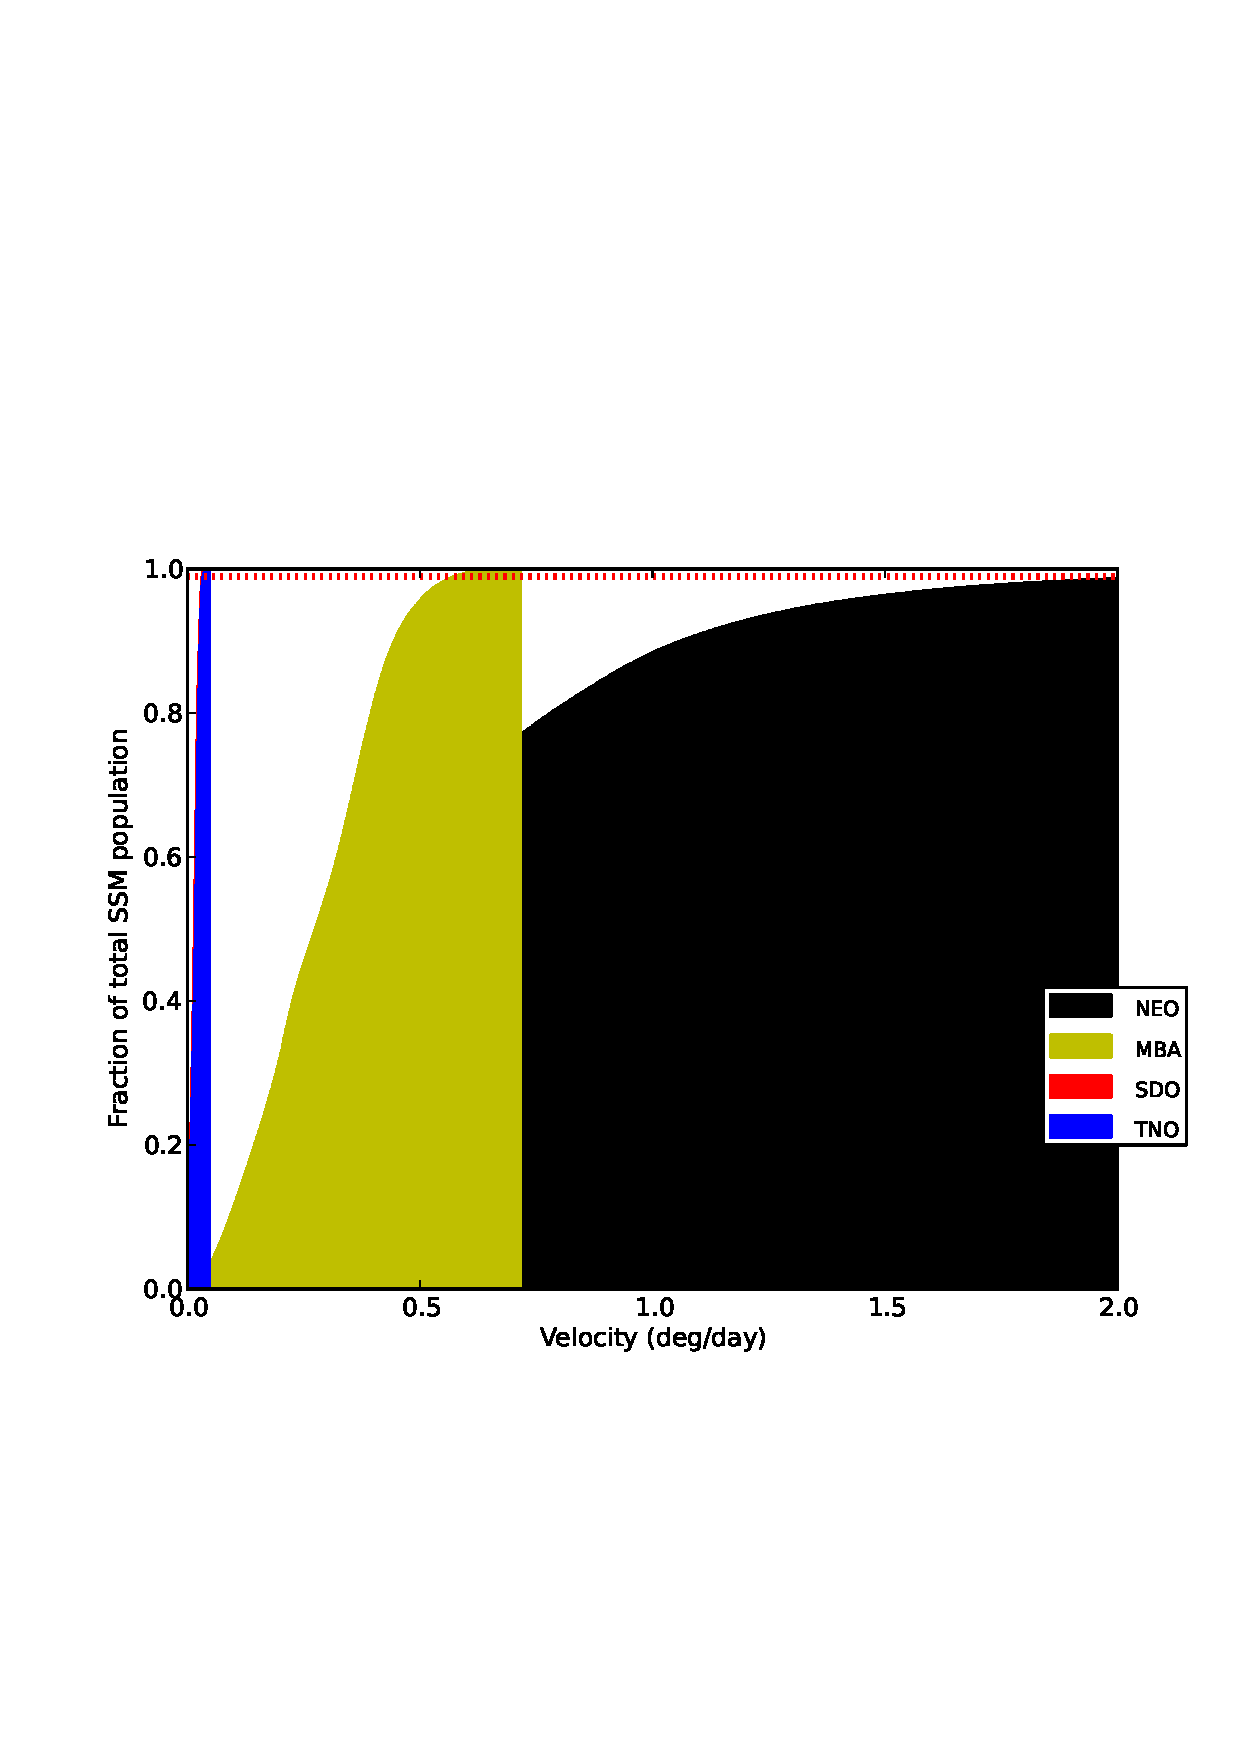
\includegraphics[width=13cm]{illustrations/mopsplots/aug2011/n_velocity.png}
  \caption[Velocity distribution of solar system objects.]{A cumulative histogram of solar solar system object
    sky-plane velocities, organized by classification.  These
    velocities include objects at all solar elongations. Classes of
    objects closer to the Sun and to the Earth (NEOs) move faster than
    objects further away (TNOs). }
  \label{velSurvey}
\end{figure}

\begin{figure}[ht!]
  \centering
  \subfloat[Apparent Accelerations in Right Ascension over 15 Days]{
    \includegraphics[width=8cm]{illustrations/mopsplots/aug2011/n_accel_ra_15.png}
    }
  \subfloat[Apparent Accelerations in Right Ascension over 30 Days]{
    \includegraphics[width=8cm]{illustrations/mopsplots/aug2011/n_accel_ra_30.png}
    }

  \subfloat[Declination Apparent Accelerations in Declination over 15 Days]{
    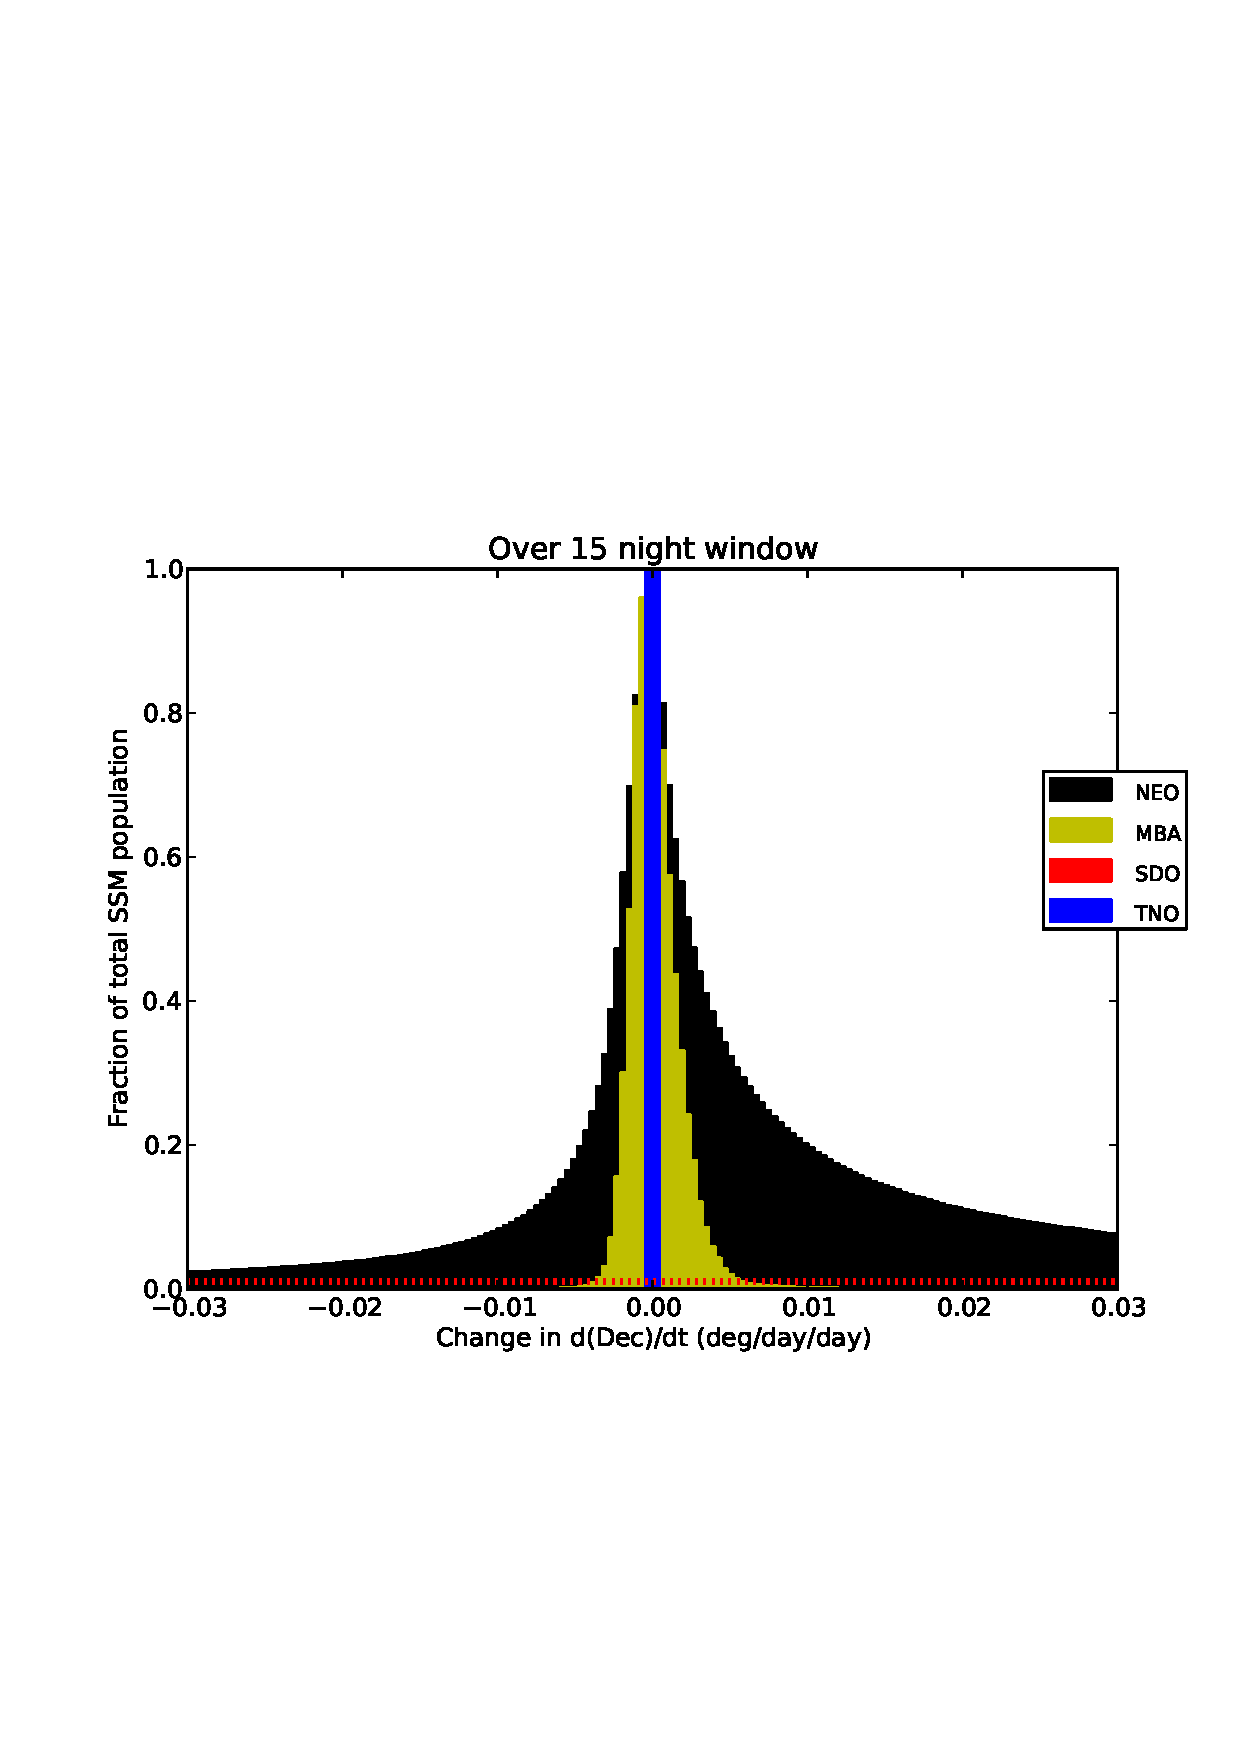
\includegraphics[width=8cm]{illustrations/mopsplots/aug2011/n_accel_dec_15.png}
    }
  \subfloat[Declination Apparent Accelerations in Declination over 30 Days]{
    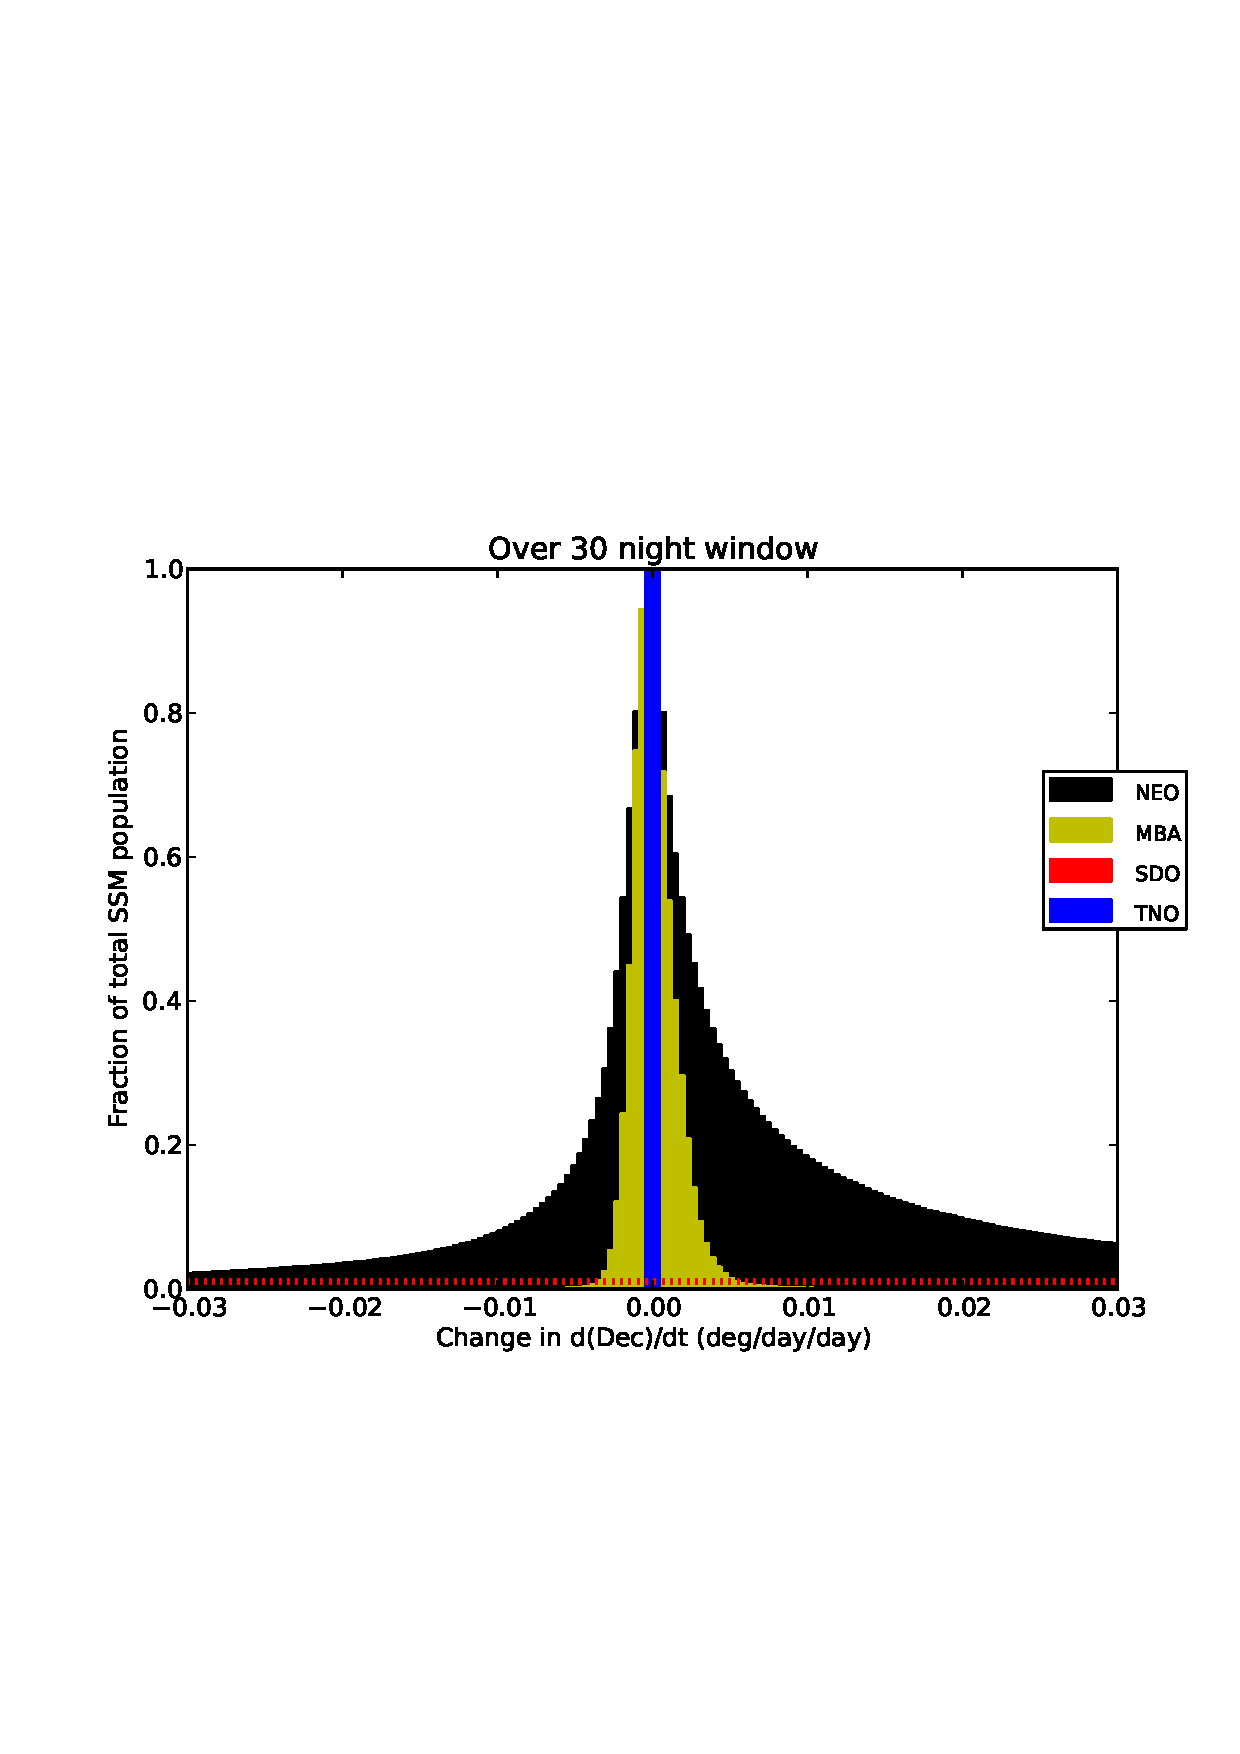
\includegraphics[width=8cm]{illustrations/mopsplots/aug2011/n_accel_dec_30.png}
    }
  \caption[Acceleration distributions of solar system objects.]{Normalized histograms of sky-plane accelerations of several
    classes solar system objects in the RA and declination, with
    objects grouped by classification.  Histograms are presented for
    changes over 15 days and 30 days. The best-fit accelerations vary
    slightly given the size of the window; this is due to
    non-quadratic factors not included in the simple quadratic model.
    15 day tracking windows are used in the experiments presented in
    this document, but we expect to move to 30 day windows in the
    future.  In both cases, virtually all MBAs, and all other objects
    except NEOs, should have accelerations between -.02 and .02
    deg/day$^2$ in both axes.}
  \label{accSurvey}
\end{figure}

We chose limits on velocity and acceleration by looking at the actual
velocities and accelerations of objects from the SSM, after generating
their ephemerides at a variety of times. Histograms of the velocities
and acceleration distributions are shown in Figures~\ref{velSurvey}
and \ref{accSurvey}. 

As can be seen from these distributions, NEOs move fastest and with
the highest accelerations, while outer solar system objects (SDOs,
TNOs) move much more slowly.  In order to detect 99\% of all MBAs,
velocity limits of 0.5 deg/day and an acceleration limit of 
.02 deg/day$^2$ are sufficient. It's worth noting that this is too
slow to detect more than about 60\% of the NEOs, but this is a
simplifying choice made to make find and linkTracklets more manageable
at this stage of development. 

By examining the detections on an object-per-object basis, we
calculated that among the 186,344 objects seen with proper cadence,
186,209 of these (more than 99.9\%) should generate useful tracks
given these velocity and acceleration limits. This is a reflection of
the fact that the overwhelming majority (about 9M of the total 11M)
objects in the SSM are MBAs, while NEOs make up only a small fraction
of solar system objects.

%% see mops64: /mnt/raid/jmyers/variousDensities/fullDensity/maxV.5_15days/trueTracks/*.log

\subsection{Simulation Results}

All simulations were conducted on the Gordon cluster at San Diego
Supercomputing Center.  Because of the large memory requirements for
running MOPS, the vSMP nodes were used for all stages of computation.
Except for the scaling tests, 16 threads were used for all the runs.


\begin{figure}[ht!]
\centering
\begin{tabular}{|r l|}
\hline
Number of asteroid detections: & 36,311,037 \\
Number of non-asteroid detections: & 0 \\
Average detections per night: & 1,134,719 \\
 & \\
Number of tracklets found: & 12,890,181 \\
Number of true tracklets: & 6,859,331 \\
Tracklets \% true: & 53.2\%\\
Tracklet generation time: & 4,791 sec (1.33 hours) \\
Tracklet generation memory use: & 13.7 GB  \\
 & \\
Number of tracks found: & 10,423,382 \\
Number of true tracks: & 5,779,424 \\
Track \% true: & 55.4\% \\
Track generation time: & 36,237 sec (10.1 hours) \\
Track generation memory use: & 16.2 GB \\
 & \\
Number of found objects: & 854,037 \\
Number of findable objects: & 1,128,643 \\
Found / findable: & 75.7\% \\
\hline
\end{tabular}

\caption[Test runs from MOPS run without noise.]{Results from the MOPS run without noise.  Velocity limit was .5 deg/day, acceleration limit was .02 deg/day$^2$ and the track chi squared probability limit was .9.  Note that not quite one fourth of objects which should generate plausible tracks are rejected.}
\label{oneMonth}
\end{figure}

\subsubsection{Survey Efficiency}

Figure~\ref{oneMonth} shows in-depth stats for a `perfect' survey,
where SSM detections above $5\sigma$ SNR in each image are reported
without additional `noise' from artifacts in difference imaging,
background transient or variable objects, or cosmic rays. 
As in all our runs, track generation is far more expensive than
tracklet generation in terms of CPU usage, but both require
substantial amounts of memory.  Also note that nearly one fourth of
the findable objects (those which should generate useful tracks) are
not found. While over time these objects may not be lost forever ({\it
  if} they are discoverable in other apparitions), this is a fairly dramatic
inefficiency in discovery rate, especially when discovery losses due
to survey cadence inefficiencies are considered. The cause of this
inefficiency is not entirely clear at present, however there are
indications it is linked to overly aggressive filtering in the
chi-squared probability filter; examining the pre-determined cutoff,
especially to see if the same cutoff should be applied over the entire
sky, would be a first step. 

Issue: This discovery rate of 75\% is a significant issue for dayMOPS
and should be investigated further. It's possible that simply tuning
the chi-squared probability filter cutoff would fix the problem,
although it could also be related to sky-plane distortion problems
once the poles are included in the input data. 

\subsubsection{Nightly Variance in Runtime}

The cost of running MOPS depends on a variety of factors which are
largely dependent on telescope operations, such as revisit rates and
the locations of revisits.  If no fields are observed that could have
compatible tracklets, then MOPS very quickly rules out these
observations and so runtime is short; on the other hand, if
having lots of potentially compatible detections means that runtime
will be longer. Figure~\ref{nightlyVariance} shows the range of
variations over the month of this simulation. 


\begin{figure}[ht!]
  \centering
  \subfloat{
    \includegraphics[width=12cm]{newIllustrations/tracklets_nightly.png}
    }
  \\
  \subfloat{
    \includegraphics[width=12cm]{newIllustrations/tracks_nightly.png}
    }

  \caption[Compute costs for tracklet and track generation.]{Per-night costs of tracklet generation and track
    generation. Also, in the track generation section,
    note that because only 31 sets of nightly tracklets were
    generated, later runs had less data in their 15-day window and thus ran
    considerably faster.  This is an artifact of the experiment and
    not a meaningful trend.}
  \label{nightlyVariance}
\end{figure}


\subsubsection{Scaling on Non-Asteroid Sources}

Actual images will contain diaSources from non-asteroid sources:
variable stars, supernova, and image processing artifacts (e.g. from
bright stars) will also be present.  Because the quality of image
processing is not known, we added non-asteroid ``noise'' detections to
images at varying rates.  At each rate, a fixed $n$ noise detections
were added to each image, with locations chosen at random. This is not
a truly realistic representation of the noise, as positions of actual
noise sources could be highly correlated and thus mimic actual moving
objects to preliminary stages of linking (thus making compute times
increase). The response of dayMOPS to actual data may thus be quite
different, but this was a reasonable starting point until more
information is available. 

We successfully ran the linking stages of dayMOPS using densities as high as 5,000 non-asteroid
sources per image.  After adding 10,000 non-asteroid sources per
image, tracklet generation was possible but linking tracklets into
tracks was too slow - at over 48 hours for a single night of
searching, it exceeded the wall-clock limit on Gordon jobs.

Figure~\ref{noiseScaling_detections} presents a short summary of the input
detection catalogs generated at each of the noise densities.  For each
of these catalogs, tracklet generation was performed for each of the
31 simulated nights of observation; results can be seen in
Figure~\ref{noiseScaling_tracklets}.  As expected, increasing numbers
of false detections lead to worse-than-linear increases in mislinkage.
This lead to worse-than-linear increases in computational costs for generating the
tracklets, both in terms of CPU and memory usage.

The tracklets generated in the tracklet generation test were used to
test scaling of track generation.  For reasons of time, we only
attempted to search for tracks starting on the first night of
observation ({\it i.e.} the first window of linkTracklets).  Results are presented in
Figure~\ref{noiseScaling_tracks} and Figure~\ref{noiseScaling_found}.
The CPU time cost for track generation scaled worse-than-linearly on
the number of tracklets.  However, we saw only modest increases in the
number of output tracks and runtime for linkTracklets, meaning that we
were able to successfully reject most of these false tracks during
track validation.  Also note that
the number of objects found remained nearly constant across the
various runs.


\begin{figure}[ht!]
\centering

\begin{tabular}{|c c c c|}
\hline
Per-Image Noise Density & Total number of detections & \% noise detections &  \\ 
0             & 36,311,037             & 0\%                          & \\
1,250         & 72,258,537             & 49.7\%          & \\
2,500         & 108,206,037            & 66.4\%          & \\ 
5,000         & 180,101,037            & 79.8\%          & \\
\hline
\end{tabular}
\caption[Input data for runs with noise.]{An overview of the detection sets used for the scaling tests on noise density.}
\label{noiseScaling_detections}
\end{figure}

\begin{figure}[ht!]
\centering

\subfloat[Number of tracklets generated at various noise density levels]
{\includegraphics[width=8cm]{newIllustrations/tracklet_num.png}}
\subfloat[Tracklet \% true at various noise density levels]
{\includegraphics[width=8cm]{newIllustrations/tracklet_true.png}}
\\
\subfloat[Tracklet generation runtimes at various noise density levels]
{\includegraphics[width=8cm]{newIllustrations/tracklet_runtime.png}}
\subfloat[Tracklet generation memory use at various noise density levels]
{\includegraphics[width=8cm]{newIllustrations/tracklet_mem.png}}

\caption[Tracklet generation for runs with noise.]{Tracklets generated at varying densities of non-asteroid
  ``noise'' sources, and corresponding compute costs.  Each data point
  represents 31 days of tracklet generation.  The same asteroid
  catalog was used for each simulation, but increasing numbers of
  ``noise'' sources were added in each simulation (see
  Figure~\ref{noiseScaling_detections}). Note that the number of
  tracklets generated, and the computational costs to find them,
  increase quickly as noise density increases. This is apparently due
  to the increase of mislinked ``false tracklets''. }
\label{noiseScaling_tracklets}
\end{figure}


\begin{figure}[ht!]
\centering

\subfloat[Number of tracks generated at various noise density levels]
{\includegraphics[width=8cm]{newIllustrations/track_num.png}}
\subfloat[Track \% true at various noise density levels]
{\includegraphics[width=8cm]{newIllustrations/track_true.png}}
\\
\subfloat[Track generation runtimes at various noise density levels]
{\includegraphics[width=8cm]{newIllustrations/track_runtime.png}}
\subfloat[Track generation memory use at various noise density levels]
{\includegraphics[width=8cm]{newIllustrations/track_mem.png}}

\caption[Track generation for runs with noise.]{Tracks generated at varying densities of non-asteroid
  ``noise'' sources, and corresponding compute costs.  Detections
  catalogs with increasing numbers of noise detections
  (Figure~\ref{noiseScaling_detections}) and tracklets generated from
  these catalogs (Figure~\ref{noiseScaling_tracklets}) were used to generate
  linkTracklets input. For reasons of time, each linkTracklets run
  attempted to find only tracks which started on the first night of
  data and ended anywhere within the first 15 days.}
\label{noiseScaling_tracks}
\end{figure}


\begin{figure}[ht!]
\centering
\begin{tabular}{|c c c|}
\hline

Noise Density & Number of Tracklets & Found Objects \\
0 & 6,312,807 & 55,982 \\
1,250 & 13,318,186 & 55,870  \\
2,500 & 25,824,121 &  55,751  \\
5,000 & 66,635,397 &  55,464  \\
\hline
\end{tabular}

\caption[Test run results for runs with noise.]{Objects found by linkTracklets with varying densities of
  noise in the input catalogs.  Note that the number of objects found
  is only slightly affected by the presence of noise in the input
  catalogs.}
\label{noiseScaling_found}
\end{figure}



\subsection{Conclusions}

For LSST images, we expect that 50-80\% of the DiaSources in our
catalogs may be attributable to non-asteroid, real astronomical sources, before
considering image subtraction artifacts.  This
corresponds to roughly 1250 or 5000 ``noise'' points per image, as we
simulated.

To meet requirements, we must be capable of running one night's-worth
of tracklet generation, track generation (using the entire previous
15 to 30 day window's worth of tracklets), and per-track IOD within 24
hours, plus precovery and attribution.  For the 50\% noise case, we saw a maximum tracklet generation
time of 10 minutes (using 16 CPUs) and for the 80\% noise case we saw
a maximum tracklet generation time of 21 minutes (again using 16
CPUs).  In our testing of track generation, we saw 306,866 tracks and
461,902 tracks generated in the 50\%-noise and 80\%-noise cases
respectively.  Expecting a trivially parallel IOD and an IOD cost of
roughly .001 seconds/track, we anticipate that IOD should not be
problematic: given a few hundred CPUs, we should be able to complete
the nightly IOD processing in a few wall-clock hours.

The cost of running linkTracklets, however, could be problematic given
the 24-hour limit.  As seen in Figure~\ref{noiseScaling_tracks} (c),
linkTracklets can be quite slow, and runtimes can increase
worse-than-linearly on the number of input tracklets, with non-linear
factors becoming significant somewhere between the 50\%-noise and
80\%-noise cases.  In the 50\%-noise experiment, runtime for a single
night was only 1.4 hours, but for the 80\%-noise experiment, runtime
was 32.5 hours!  Again, both experiments used 16 CPUs.  

In our one-month run of linkTracklets without noise, we found the
per-night cost of tracklet generation could vary by a factor of two or
more (see Figure~\ref{nightlyVariance}).  Applying this to the runs performed with noise, this gives us
an estimated maximum nightly runtime of between 2.8 and 65
hours (assuming 16 CPUs).

In order to reach the goal of running tracklet generation, track
generation, and IOD on the tracks, we should aim to reduce the maximum
runtime of linkTracklets to below 20 hours in the worst case.  This
requires a speedup of at least 3-4 over the current performance.  Such
a speedup may be possible simply by waiting on Moore's law, but it would be preferable to begin experimenting with
larger numbers of threads and possible sequential optimizations as
soon as possible, together with looking at potential improvements in
the uderlying KD-Tree algorithms (such as optimizing the tree-walking
code, making sure the leaf-node sizes are appropriate, checking
support node splitting, and ensuring that memory is being accessed
efficiently. It may also be worthwhile to explore GPUs in the context
of parallelization, if trees can be efficiently split between
different machines to reduce individual memory footprint
requirements (such as was attempted with the preliminary work on a
distributed linkTracklets algorithm by Matt Cleveland). 

Preliminary scaling experiments showed little additional speedup when
using more than 16 CPUs, and a possible slowdown as the number of CPUs
exceeded 20.  However, these tests were conducted using a smallish
data set, and should be repeated with a larger one.  Initial tests
were also conducted on Gordon vSMP nodes, which hold only 16 CPUs per
motherboard; this is another possible cause of the poor scaling beyond
16 CPUs, and should be compared with scaling tests on conventional
single-board, large-memory UMA machines.
